\documentclass{article}

% 导入宏包
\usepackage{fancyhdr}
\usepackage{ctex}
\usepackage{listings}
\usepackage{graphicx}
\usepackage[a4paper, body={18cm,22cm}]{geometry}
\usepackage{amsmath,amssymb,amstext,wasysym,enumerate,graphicx}
\usepackage{float,abstract,booktabs,indentfirst,amsmath}
\usepackage{array}
\usepackage{multirow}
\usepackage{url}
\usepackage{diagbox}
\usepackage{enumitem}
\usepackage{xcolor}
\usepackage{makecell}
\usepackage{tikz}
\usetikzlibrary{positioning, arrows.meta}

% 设置段落
\renewcommand\arraystretch{1.4}
\setlength{\parindent}{2em}
\setCJKmonofont{黑体}

% 配置代码显示
\lstset{
	xleftmargin = 3em,
	xrightmargin = 3em,
	aboveskip = 1em,
	backgroundcolor = \color{white},
	basicstyle = \small\ttfamily,
	rulesepcolor = \color{gray},
	breaklines = true,
	numbers = left,
	numberstyle = \small,
	numbersep = -14pt,
	keywordstyle = \color{purple}\bfseries,
	commentstyle = \color{green!60!black}, % 修改注释颜色
	stringstyle = \color{red!60!green!90!blue!90},
	morekeywords = {ASSERT, int64_t, uint32_t},
	moreemph = {ASSERT, NULL},
	emphstyle = \color{red}\bfseries,
	moreemph = [2]{int64\_t, uint32\_t, tid\_t, uint8\_t, int16\_t, uint16\_t, int32\_t, size\_t, bool},
	emphstyle = [2]\color{purple}\bfseries,
	frame = shadowbox,
	showspaces = false,
	columns = fixed
	morecomment = [l][\color{green!60!black}]{+}, % 设置以+开头的代码行为绿色
}

%--------------------页眉--------------------%

\pagestyle{fancy}
\fancyhead[L]{}
\fancyhead[R]{}
\fancyhead[C]{华东师范大学软件工程学院实验报告}
\fancyfoot[C]{-\thepage-}
\renewcommand{\headrulewidth}{1.5pt}

%--------------------标题--------------------%

\begin{document}
	\begin{center}
		{\Large{\textbf{\heiti 华东师范大学软件工程学院实验报告}}}
		\begin{table}[htb]
			\flushleft
			\begin{tabular}{p{0.4\linewidth}p{0.27\linewidth}p{0.28\linewidth}}\\
				\textbf{实验课程}:计算机网络实践  & \textbf{年级}:2023级       & \textbf{实验成绩}:  \\
				\textbf{实验名称}:Ethernet & \textbf{姓名}:顾翌炜         &                 \\
				\textbf{实验编号}:Lab-2     & \textbf{学号}:10235101527 & \textbf{实验日期}:2024/11/29  \\
				\textbf{指导教师}:王廷     & \textbf{组号}:01            & \textbf{实验时间}:2024/11/29  \\ 
			\end{tabular}
		\end{table}
	\end{center}
	\rule{\textwidth}{2pt}
	
	%--------------------正文--------------------%
	\section{实验目的}
	
	\begin{enumerate}[noitemsep, label={{\arabic*})}]
		\item 学会通过Wireshark获取以太网的帧
		\item 掌握以太网的结构
		\item 分析以太网地址范围
		\item 分析以太网的广播帧
	\end{enumerate}
	
	\section{实验内容和实验步骤}
	
	\subsection{实验内容}
	
	\subsubsection{获取以太网的帧}
	
	在cmd中使用\texttt{ping}命令发起\texttt{ICMP}请求,然后使用\texttt{Wireshark}捕获以太网数据包。
	
	\subsubsection{分析以太网的帧}
	
	分析\textbf{以太网}的帧,画出帧结构。
	
	\subsubsection{分析以太网的地址范围}
	
	分析\textbf{以太网}的地址范围,画出图示关系图。
	
	\subsubsection{分析以太网的广播帧}
	
	启动\texttt{Wireshark},在菜单栏的捕获\texttt{→}选项中进行设置,选择已连接的以太网,设置捕获过滤器为\texttt{ethermulticast},捕获以太网的广播帧。
	
	分析以太网的广播帧,回答以下问题:
	
	\begin{enumerate}[noitemsep, label={{\arabic*})}]
		\item What is the broadcast Ethernet address, written in standard form as Wireshark displays it?
		\item Which bit of the Ethernet address is used to determine whether it is unicast or multicast/broadcast?
	\end{enumerate}
	
	\subsubsection{问题讨论}
	
	\begin{enumerate}[noitemsep, label={{\arabic*})}]
		\item How long are the combined IEEE 802.3 and LLC headers compared to the DIX Ethernet headers? You can use Wireshark to work this out. Note that the Trailer/Padding and Checksum may be shown as part of the header, but they come at the end of the frame.
		\item How does the receiving computer know whether the frame is DIX Ethernet or IEEE 802.3? Hint: you may need to both use Wireshark to look at packet examples and read your text near where the Ethernet formats are described.
		\item If IEEE 802.3 has no Type field, then how is the next higher layer determined? Use Wireshark to look for the demultiplexing key.
	\end{enumerate}
	
	\subsection{实验步骤}
	
	\begin{enumerate}[noitemsep, label={{\arabic*})}]
		\item 打开cmd,使用\texttt{ping www.baidu.com}命令来发起ICMP请求
		\item 启动\texttt{Wireshark},在菜单栏捕获 \texttt{→} 选项重的设置,选择已连接的以太网,设置捕获过滤器为icmp,将混杂模式设置为关闭,勾选\texttt{enable MAC name resolution},然后开始捕获
		\item 回到cmd,再次使用\texttt{ping www.baidu.com}发起ICMP请求
		\item 回到\texttt{Wireshark},停止捕获
		\item 分析捕获到的以太网的帧,画出帧结构
		\item 分析以太网的地址范围,画出图示关系图
		\item 启动\texttt{Wireshark},在菜单栏捕获 \texttt{→} 选项重的设置,选择已连接的以太网,设置捕获过滤器为\texttt{ether multicast},然后开始捕获以太网的广播帧。
		\item 问题讨论
	\end{enumerate}
	
	\section{实验环境}

	\begin{itemize}[noitemsep]
		\item 操作系统:\texttt{Windows 11 家庭中文版 23H2 22631.4460}
		\item 网络适配器:\texttt{Killer(R)Wi-Fi 6E AX1675i 160MHz Wireless Network Adapter(211NGW)}
		\item \texttt{Wireshark}:\texttt{Version 4.4.1}
		\item \texttt{wget}:\texttt{GNU Wget 1.21.4 built on mingw32}
	\end{itemize}

	\section{实验过程与分析}
	
	\subsection{获取以太网的帧}
	
	首先,我们在命令行中使用\texttt{ping}命令发起\texttt{ICMP}请求。
	
	\begin{lstlisting}[language=bash]
        C:\User\GHOST> ping www.baidu.com
	\end{lstlisting}
	
	\begin{figure}[H]
		\centering
		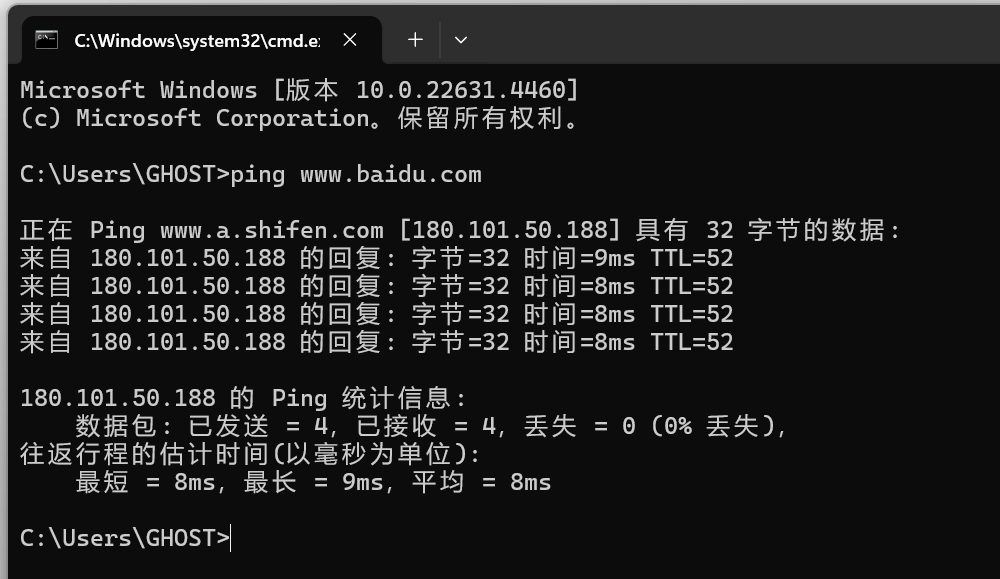
\includegraphics[width=11cm]{images/1.使用ping命令发起ICMP请求.jpg}
		\caption{使用ping命令发起ICMP请求}
	\end{figure}
	
	启动\texttt{Wireshark},在菜单栏捕获 \texttt{→} 选项重的设置,选择已连接的以太网,设置捕获过滤器为icmp,将混杂模式设置为关闭,勾选\texttt{enable MAC name resolution},然后开始捕获
	
	\begin{figure}[H]
		\centering
		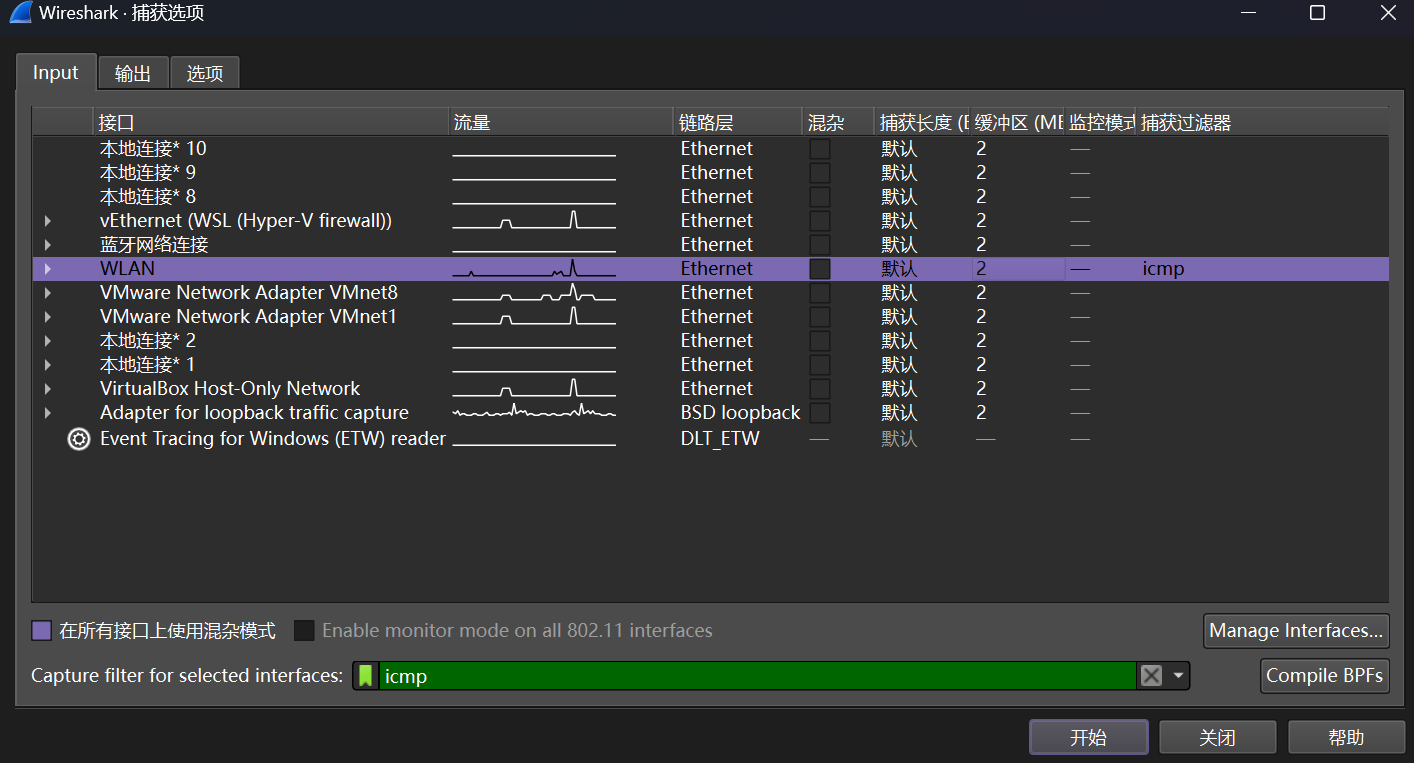
\includegraphics[width=11cm]{images/2.设置Wireshark捕获过滤器.png}
		\caption{设置Wireshark捕获过滤器}
	\end{figure}
	
	回到cmd,再次使用\texttt{ping www.baidu.com}发起ICMP请求
	
	\begin{figure}[H]
		\centering
		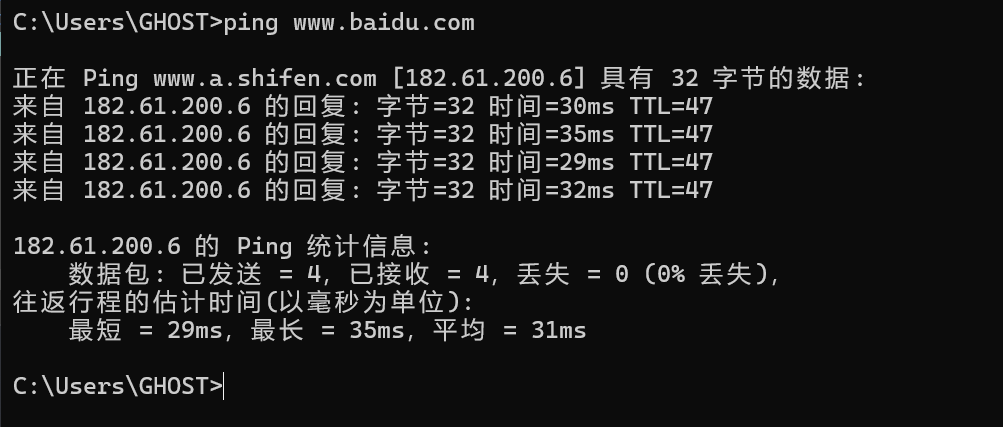
\includegraphics[width=11cm]{images/3.再次发起ICMP请求.png}
		\caption{再次发起ICMP请求}
	\end{figure}
	
	回到\texttt{Wireshark},停止捕获,得到的结果如下图所示:
	
	\begin{figure}[H]
		\centering
		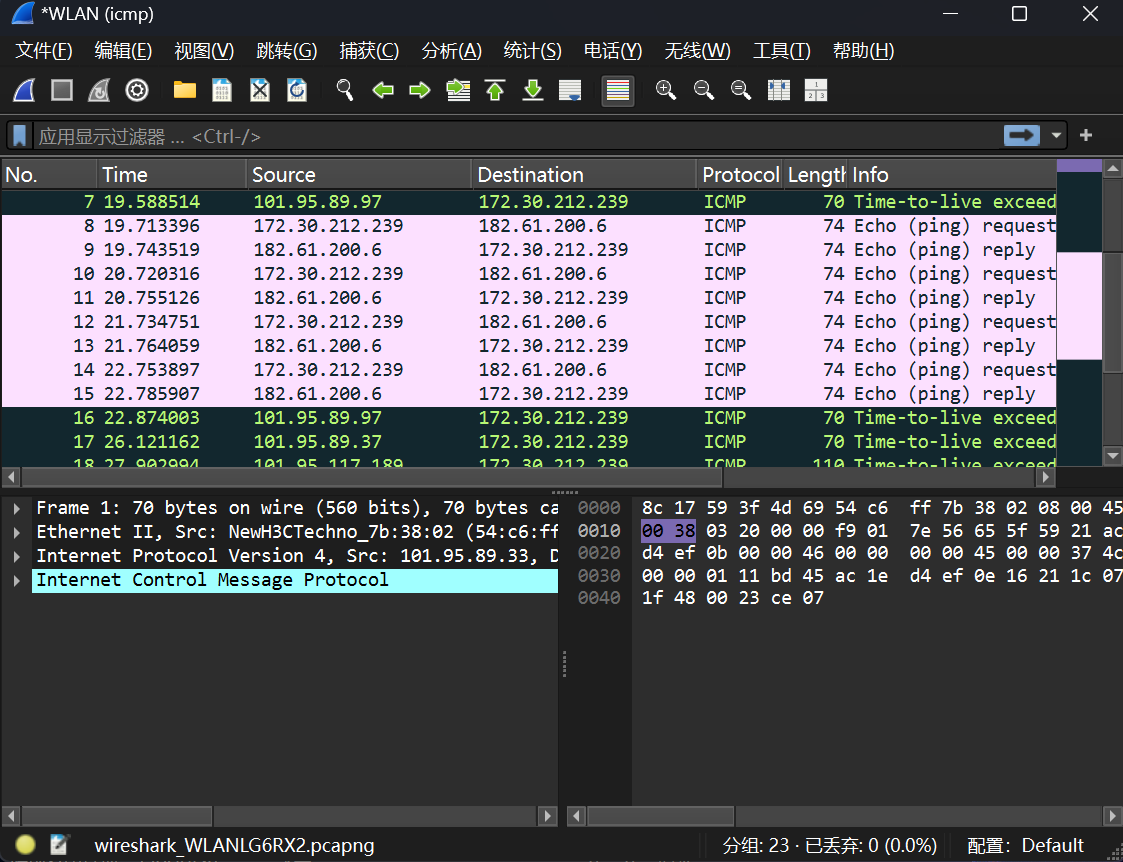
\includegraphics[width=11cm]{images/4.捕获结果.png}
		\caption{捕获结果}
	\end{figure}
	
	\subsection{分析以太网的帧}
	
	点击捕获到的数据包,选择\textbf{Ethernet II},可以看到以太网的帧结构如下图所示:
	
	\begin{figure}[H]
		\centering
		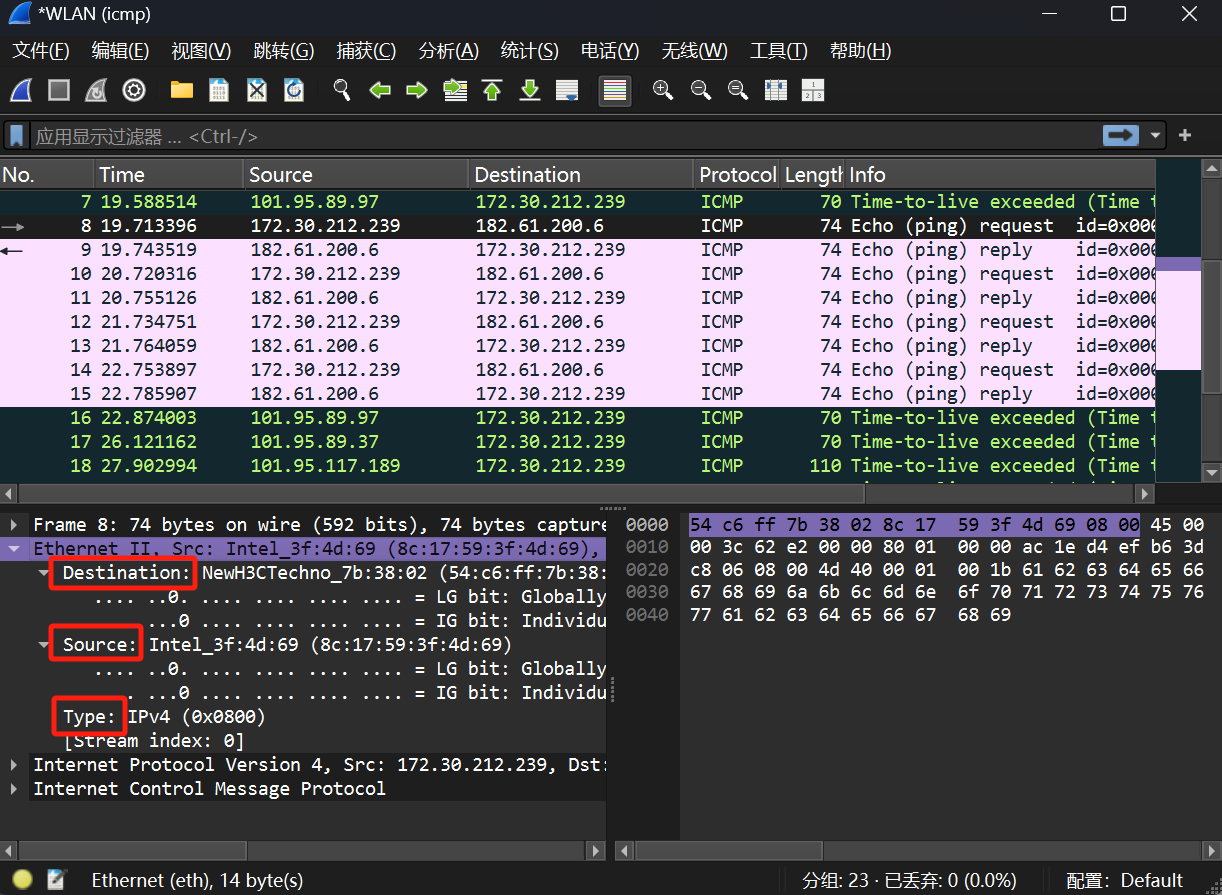
\includegraphics[width=11cm]{images/5.以太网的帧结构.png}
		\caption{以太网的帧结构}
	\end{figure}
	
	以太网的帧结构中包含了:目的地址\textbf{Destination}, 源地址\textbf{Source}, 类型\textbf{Type}等内容。
	
	其中目的地址和源地址都是\textbf{6}个字节,类型是\textbf{2}个字节。
	
	\begin{figure}[H]
		\centering
		\begin{minipage}[b]{0.45\textwidth}
			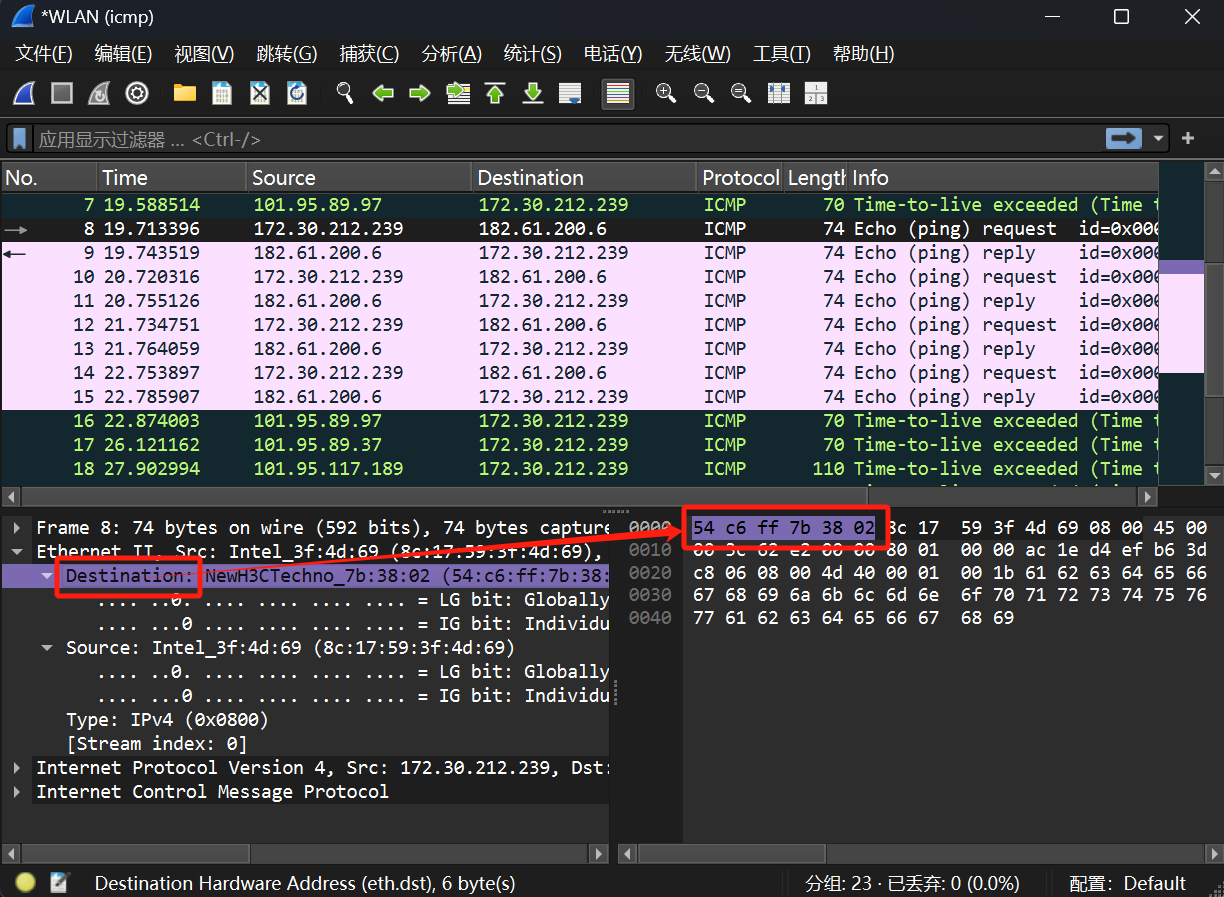
\includegraphics[width=\textwidth]{images/6.Destination.png}
			\caption{Destination}
		\end{minipage}
		\hfill
		\begin{minipage}[b]{0.45\textwidth}
			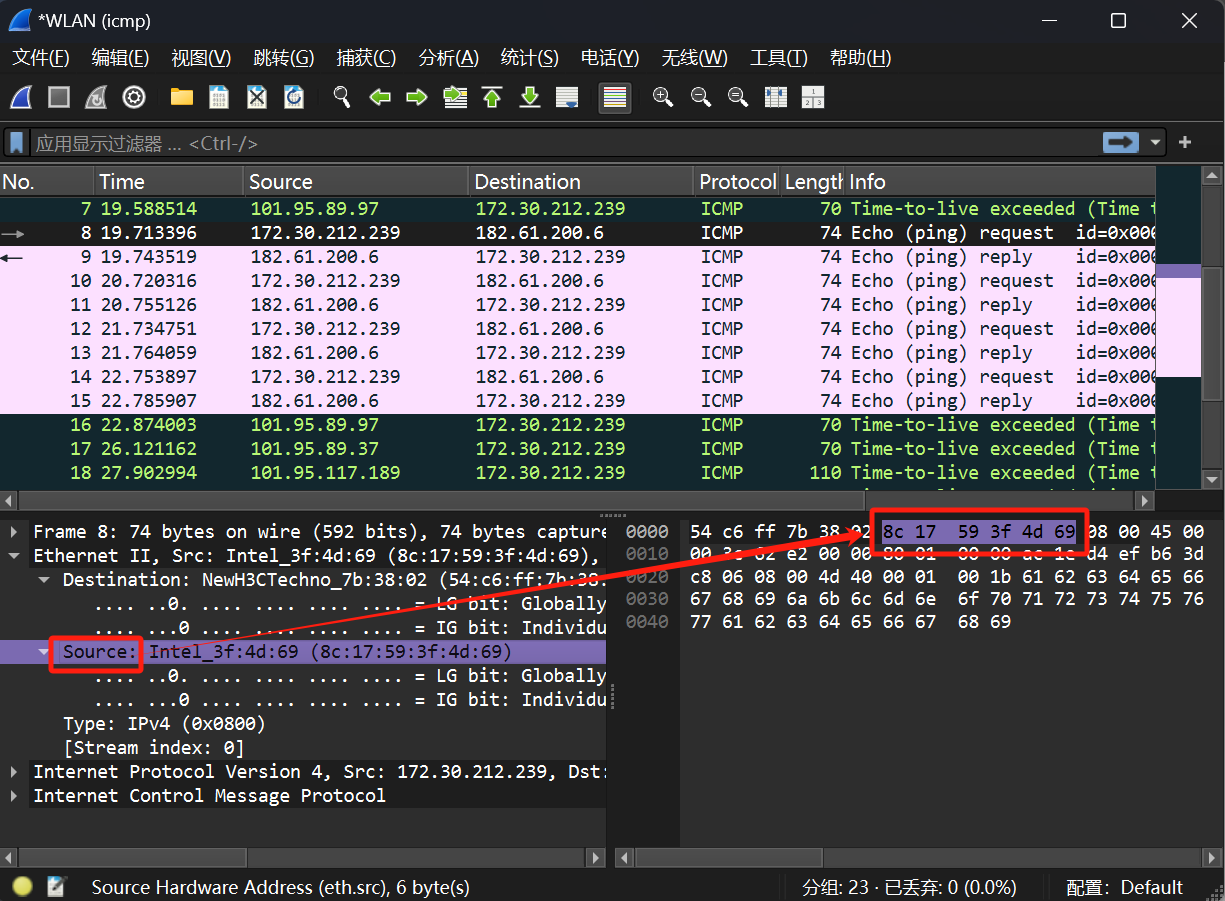
\includegraphics[width=\textwidth]{images/7.Source.png}
			\caption{\texttt{Source}}
		\end{minipage}
	\end{figure}
	
	\begin{figure}[H]
		\centering
		\begin{minipage}[b]{0.45\textwidth}
			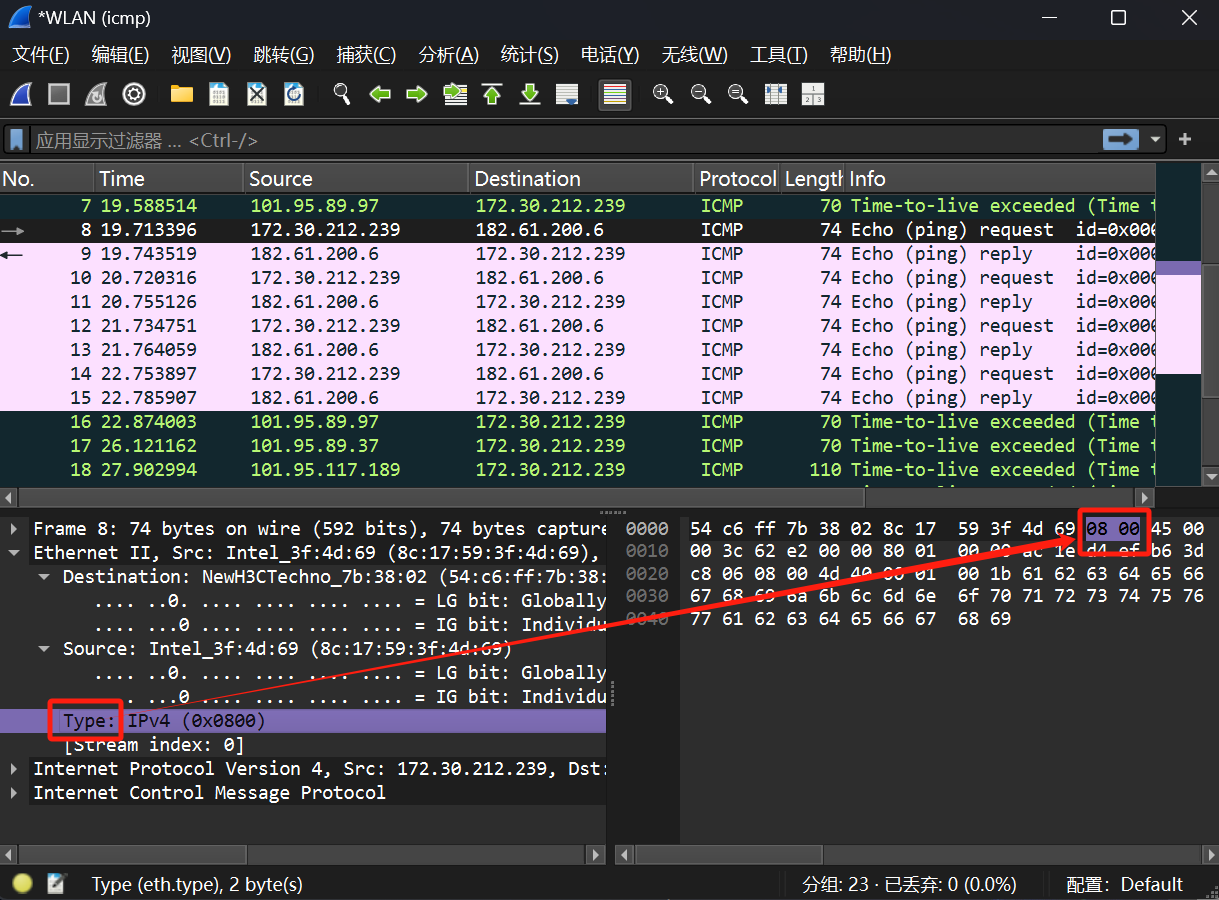
\includegraphics[width=\textwidth]{images/8.Type.png}
			\caption{Type}
		\end{minipage}
	\end{figure}
	
	再通过观察,找到checksum内容为correct:
	
	\begin{figure}[H]
		\centering
		\begin{minipage}[b]{0.45\textwidth}
			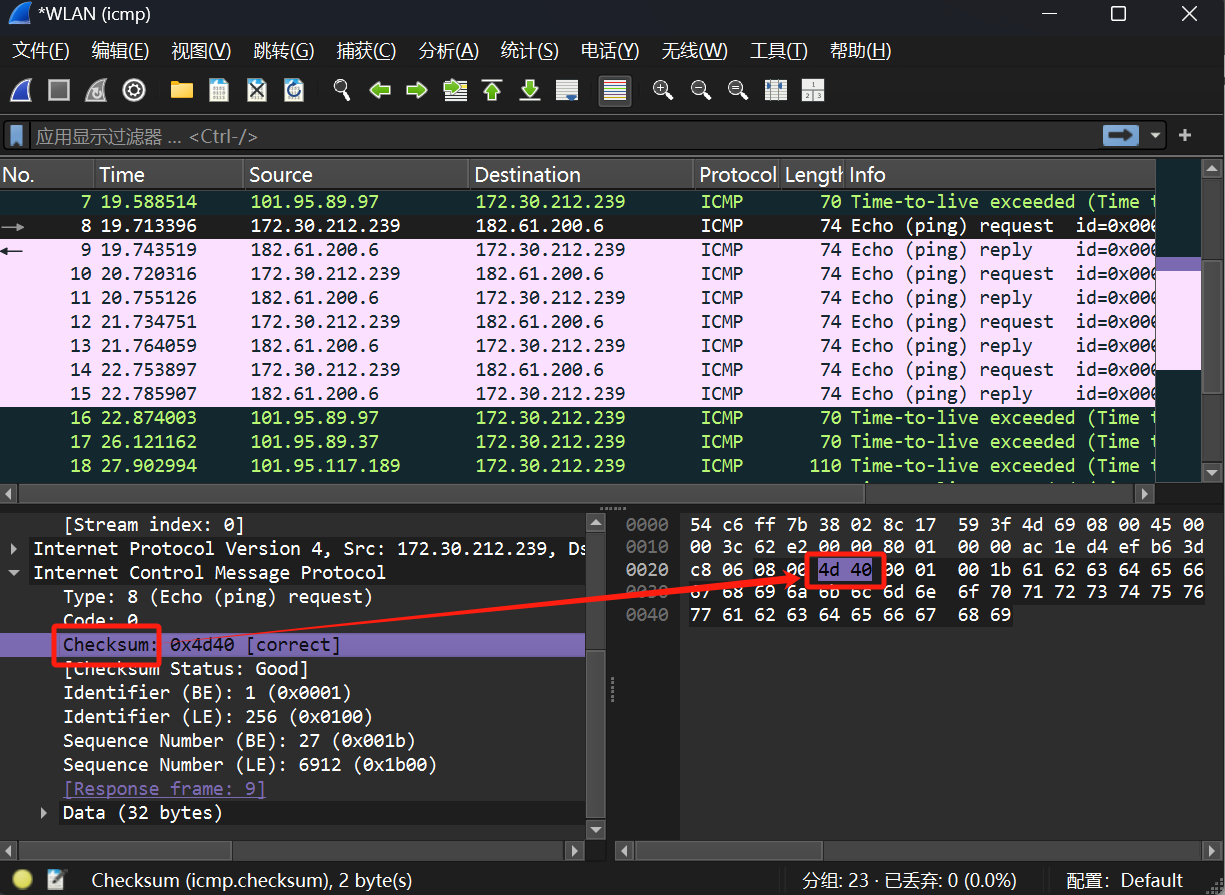
\includegraphics[width=\textwidth]{images/9.checksum.png}
			\caption{checksum}
		\end{minipage}
	\end{figure}
	
	由此画出来的帧结构如图所示:
	
	\begin{figure}[H]
		\centering
		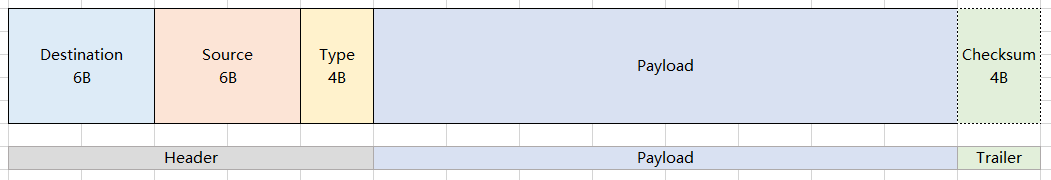
\includegraphics[width=15cm]{images/12.以太网帧结构.jpg}
		\caption{以太网帧结构}
	\end{figure}
	
	\subsection{分析以太网的地址范围}
	
	再结合以下信息:
	
	\begin{figure}[H]
		\centering
		\begin{minipage}[b]{0.45\textwidth}
			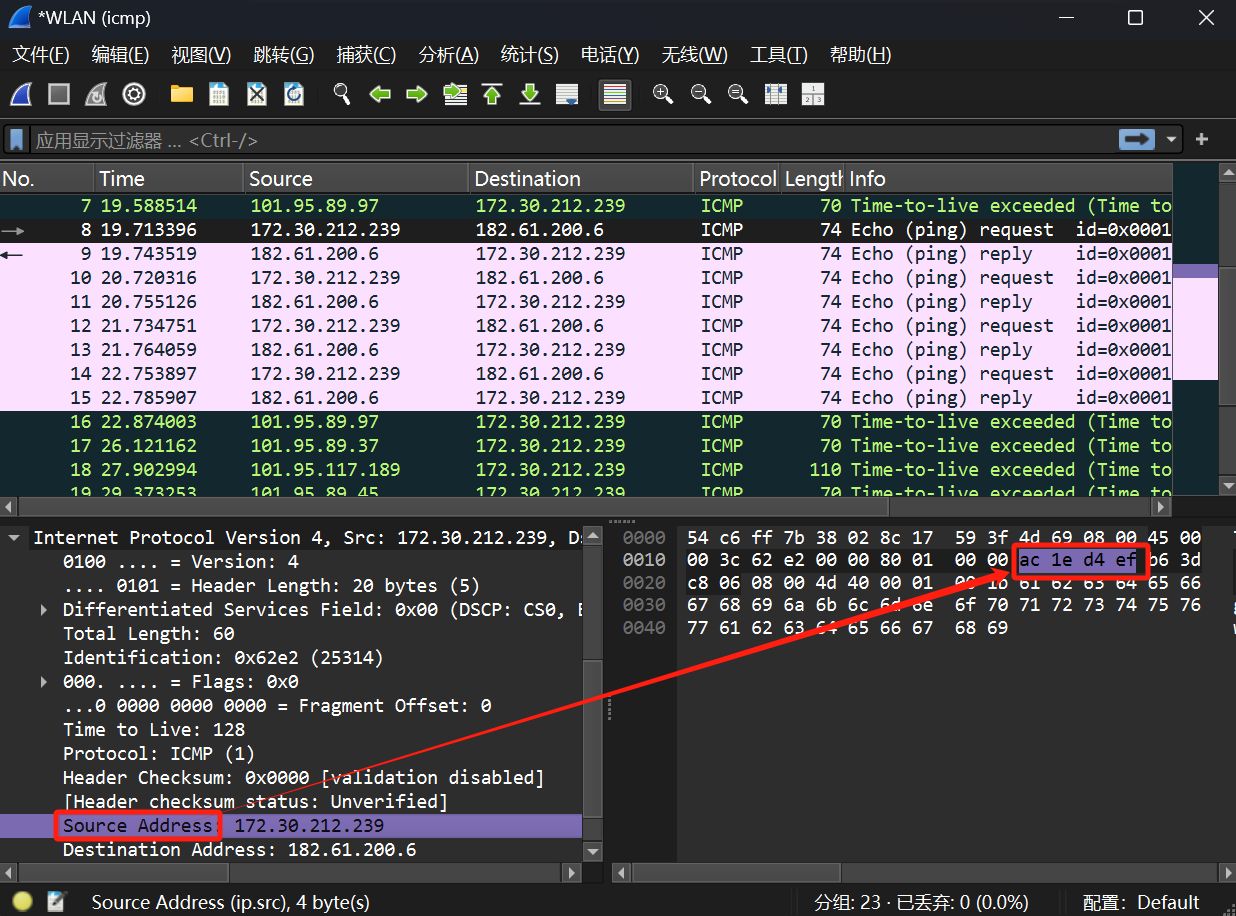
\includegraphics[width=\textwidth]{images/10.source的IP.png}
			\caption{source的IP}
		\end{minipage}
		\hfill
		\begin{minipage}[b]{0.45\textwidth}
			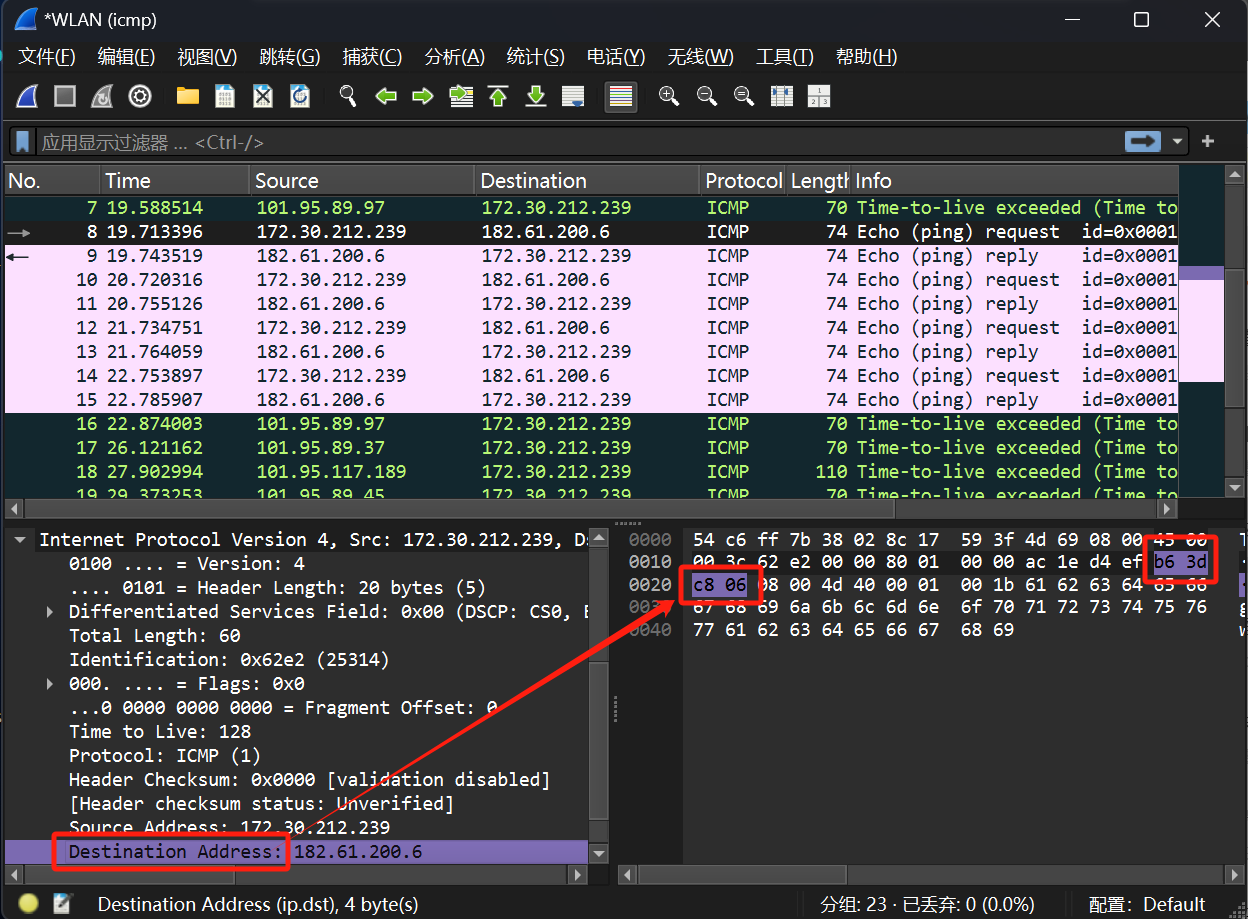
\includegraphics[width=\textwidth]{images/11.destination的IP.png}
			\caption{\texttt{destination的IP}}
		\end{minipage}
	\end{figure}
	
	根据上面分析得到的以太网帧结构,我们可以得知本机MAC地址为8c:17:59:3f:4d:69,IP地址为172.30.212.239,路由器MAC地址为54:c6:ff:7b:38:02,目标IP地址为: 182.61.200.6。
	
	可以作出如下的关系图:
	
	\begin{figure}[H]
		\centering
		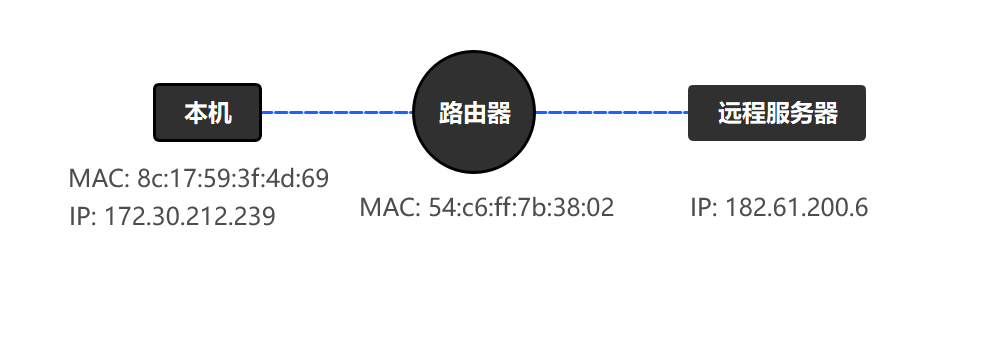
\includegraphics[width=15cm]{images/13.以太网地址范围关系图.png}
		\caption{以太网地址范围关系图}
	\end{figure}
	
	\subsection{分析以太网的广播帧}
	
	启动\texttt{Wireshark},在菜单栏捕获 \texttt{→} 选项重的设置,选择已连接的以太网,设置捕获过滤器为\texttt{ether multicast},然后开始捕获以太网的广播帧。
	
	\begin{figure}[H]
		\centering
		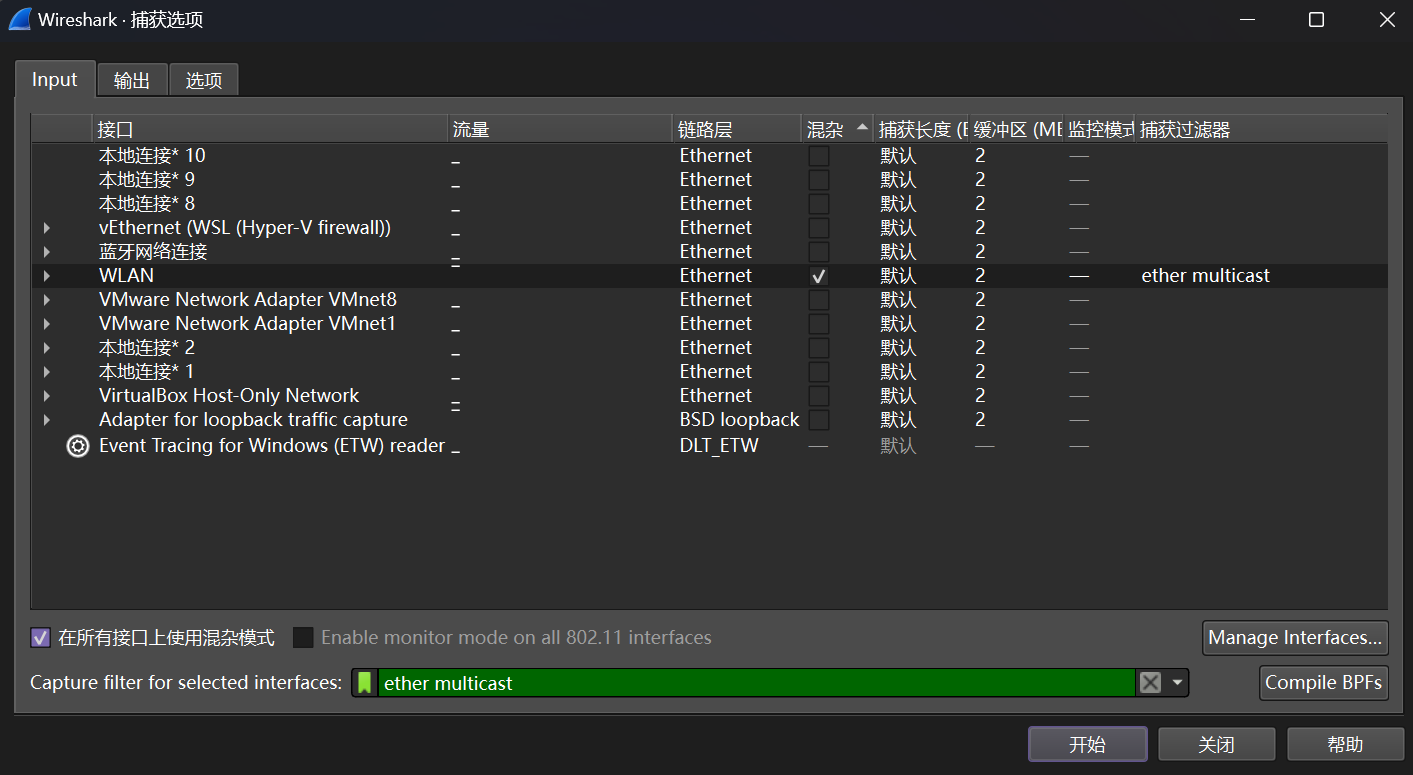
\includegraphics[width=11cm]{images/14.设置Wireshark捕获过滤器.png}
		\caption{设置Wireshark捕获过滤器}
	\end{figure}
	
	持续捕获一段时间之后,捕获结果如下图所示:
	
	\begin{figure}[H]
		\centering
		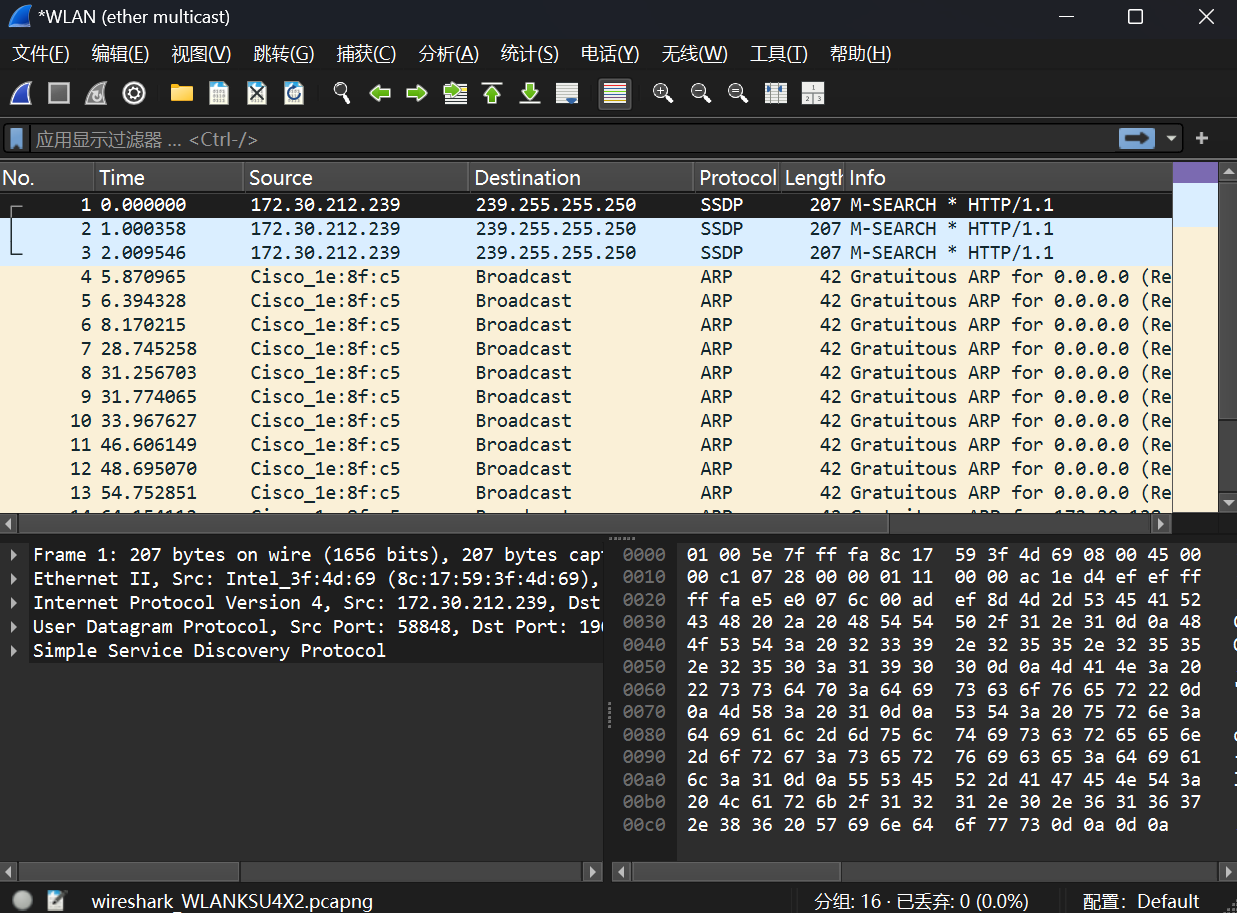
\includegraphics[width=11cm]{images/15.捕获结果.png}
		\caption{捕获结果}
	\end{figure}
	
	选择其中的一个广播帧数据包,如下图所示:
	
	\begin{figure}[H]
		\centering
		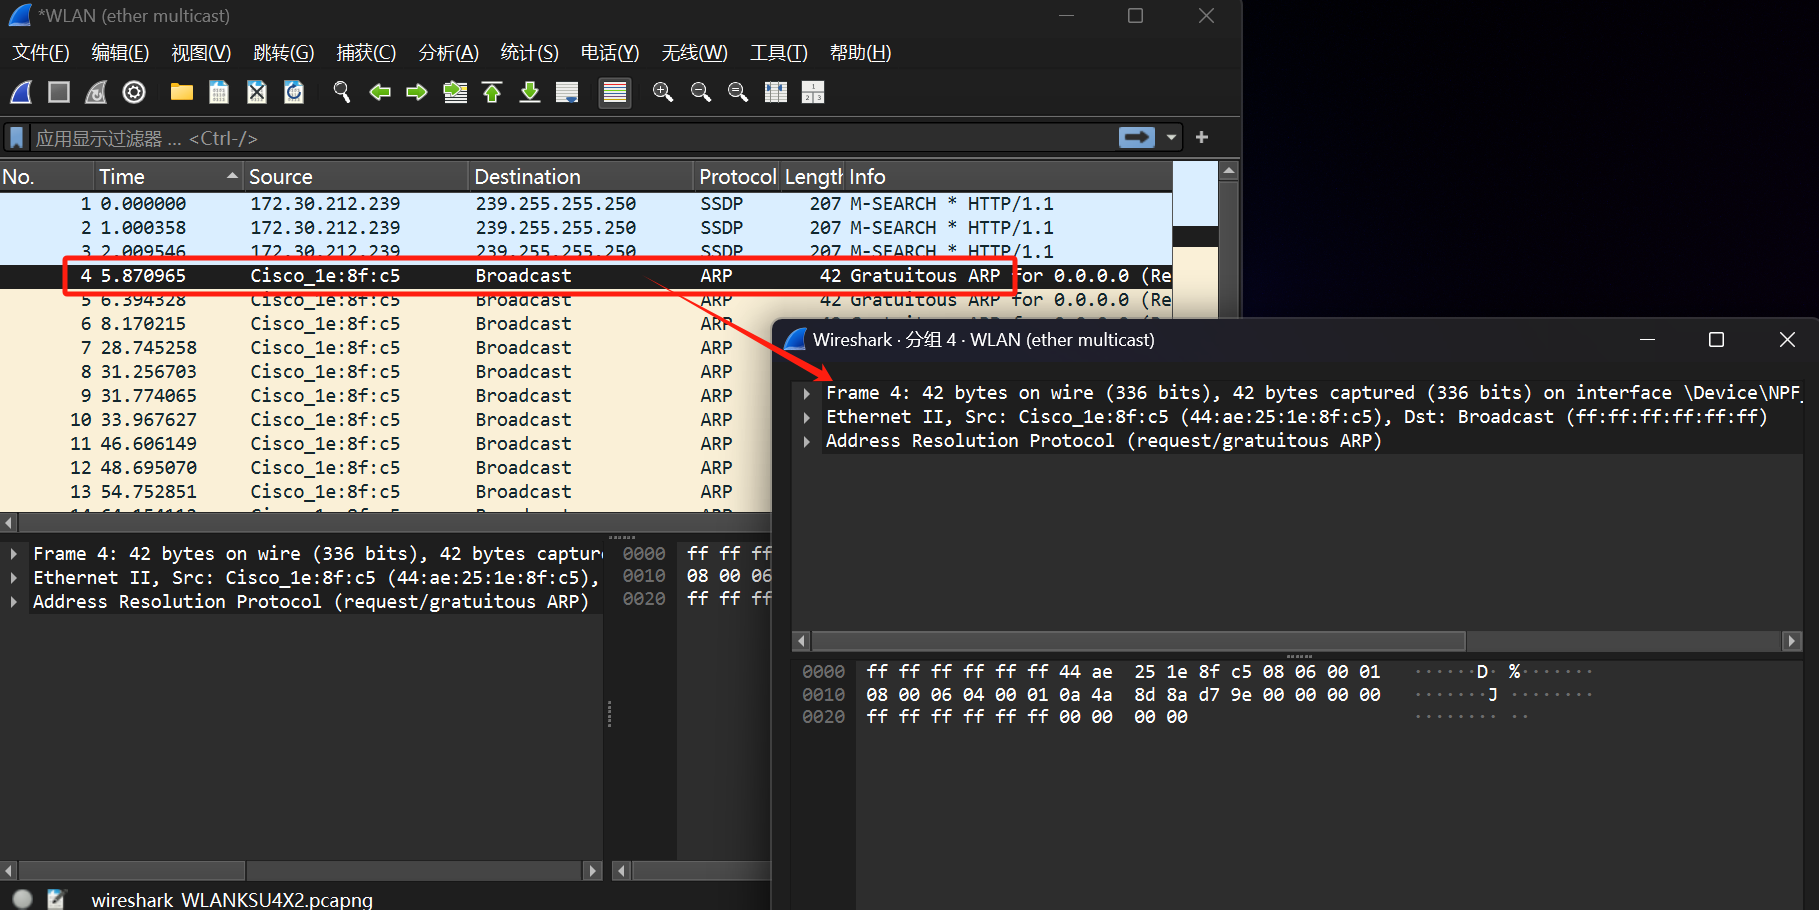
\includegraphics[width=11cm]{images/16.广播帧数据包.png}
		\caption{广播帧数据包}
	\end{figure}
	
	接下来开始分析问题:
	
	1. 以太网广播帧的地址是什么, 以标准的形式写在Wireshark上显示?
	
	\begin{figure}[H]
		\centering
		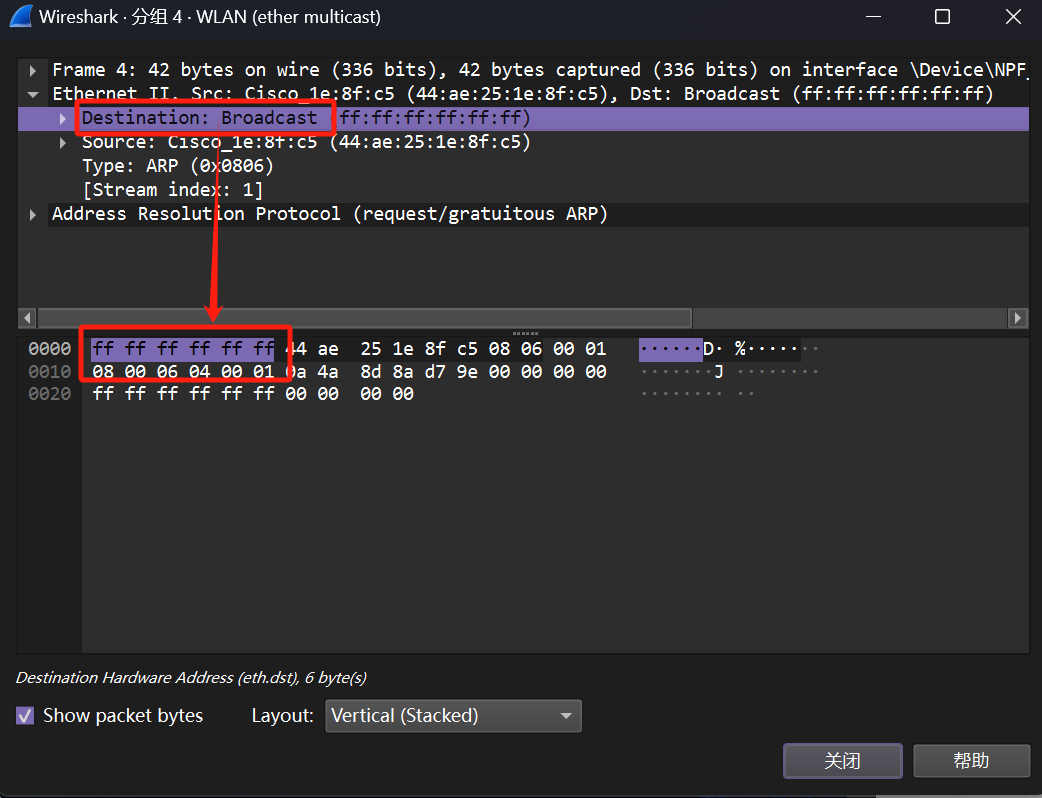
\includegraphics[width=11cm]{images/17.广播帧地址.png}
		\caption{广播帧地址}
	\end{figure}
	
	可以看出:广播帧的地址为ff:ff:ff:ff:ff:ff。
	
	2. 哪几个比特位的以太网地址是用来确定是单播或多播/广播?
	
	\begin{figure}[H]
		\centering
		\begin{minipage}[b]{0.45\textwidth}
			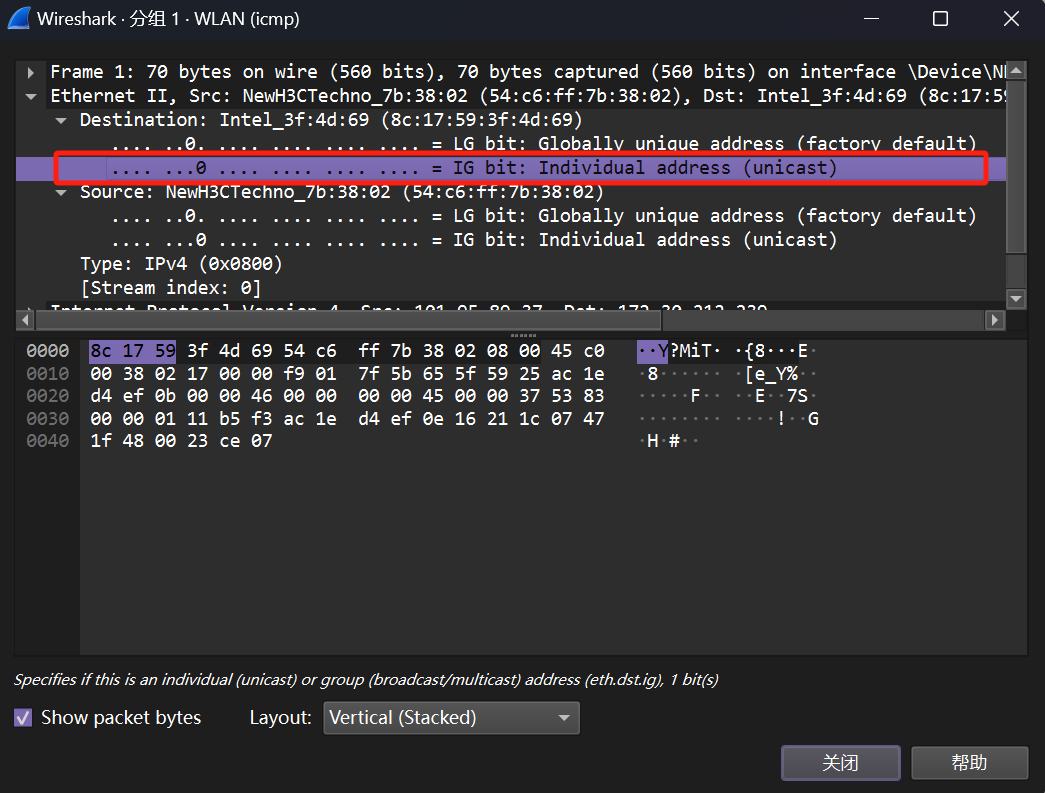
\includegraphics[width=\textwidth]{images/18.单播帧.png}
			\caption{单播帧}
		\end{minipage}
		\hfill
		\begin{minipage}[b]{0.45\textwidth}
			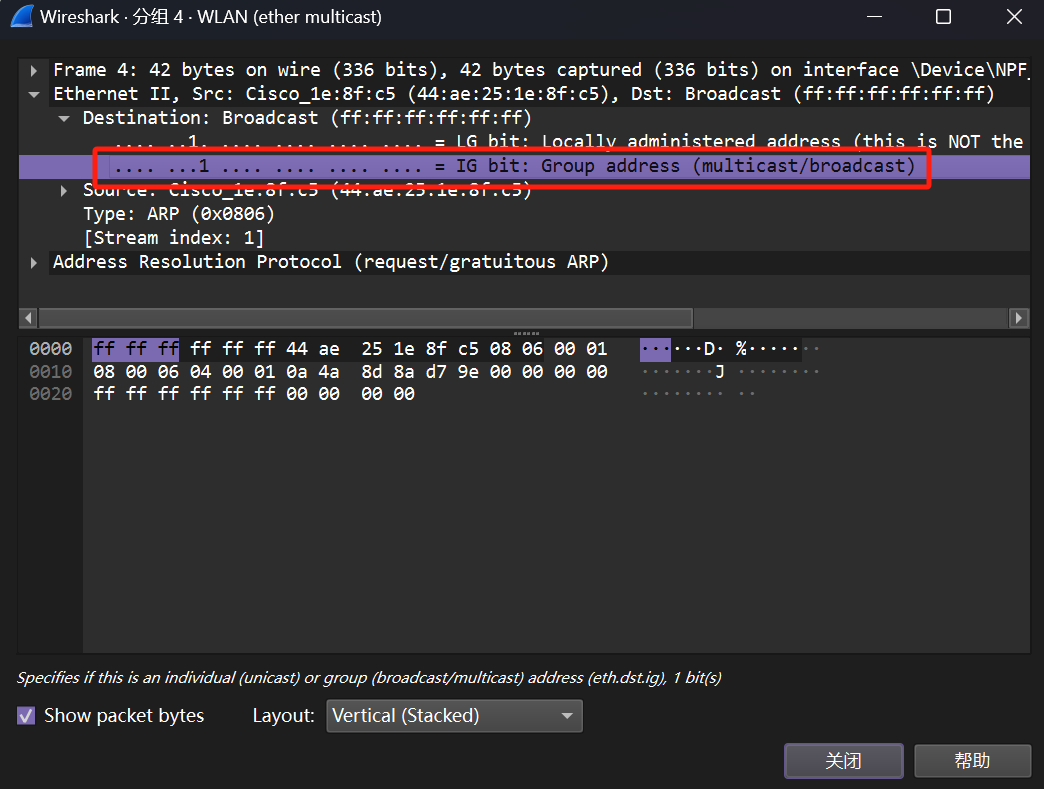
\includegraphics[width=\textwidth]{images/19.广播帧.png}
			\caption{\texttt{广播帧}}
		\end{minipage}
	\end{figure}
	
	对比单播帧和广播帧(如上图所示)可以看出,以太网地址的第一个字节的最后一位(即第八位)为1,所以可以确定是多播/广播。
	
	\subsection{问题讨论}
	
	由于抓包了很久一直都没有抓到以太网的帧,所以这里直接使用实验手册里的那份数据来分析。
	
	设置捕获过滤器为llc,捕获以太网的帧,如下图所示:
	
	\begin{figure}[H]
		\centering
		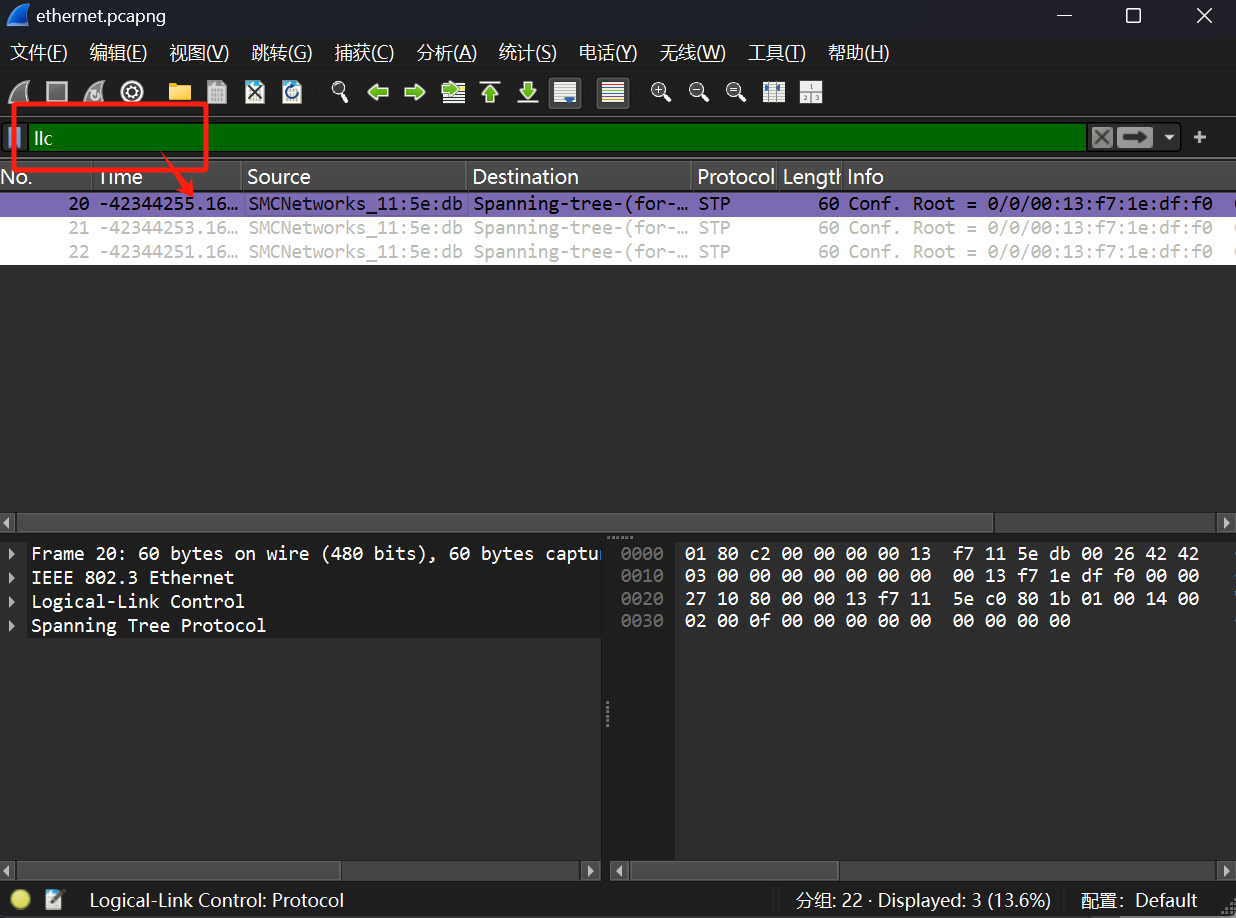
\includegraphics[width=11cm]{images/20.捕获IEEE802.3以太网的帧.png}
		\caption{捕获IEEE802.3以太网的帧}
	\end{figure}
	
	\begin{enumerate}[noitemsep, label={{\arabic*})}]
		\item How long are the combined IEEE 802.3 and LLC headers compared to the DIX Ethernet headers? You can use Wireshark to work this out. Note that the Trailer/Padding and Checksum may be shown as part of the header, but they come at the end of the frame.\\
		
		根据下图所显示:可以看到:\textbf{IEEE 802.3}头部长度为\texttt{14}字节,\textbf{LLC}头部长度为\texttt{3}字节(\textbf{DIX}以太网头部长度为\texttt{14}字节)
		
		\begin{figure}[H]
			\centering
			\begin{minipage}[b]{0.45\textwidth}
				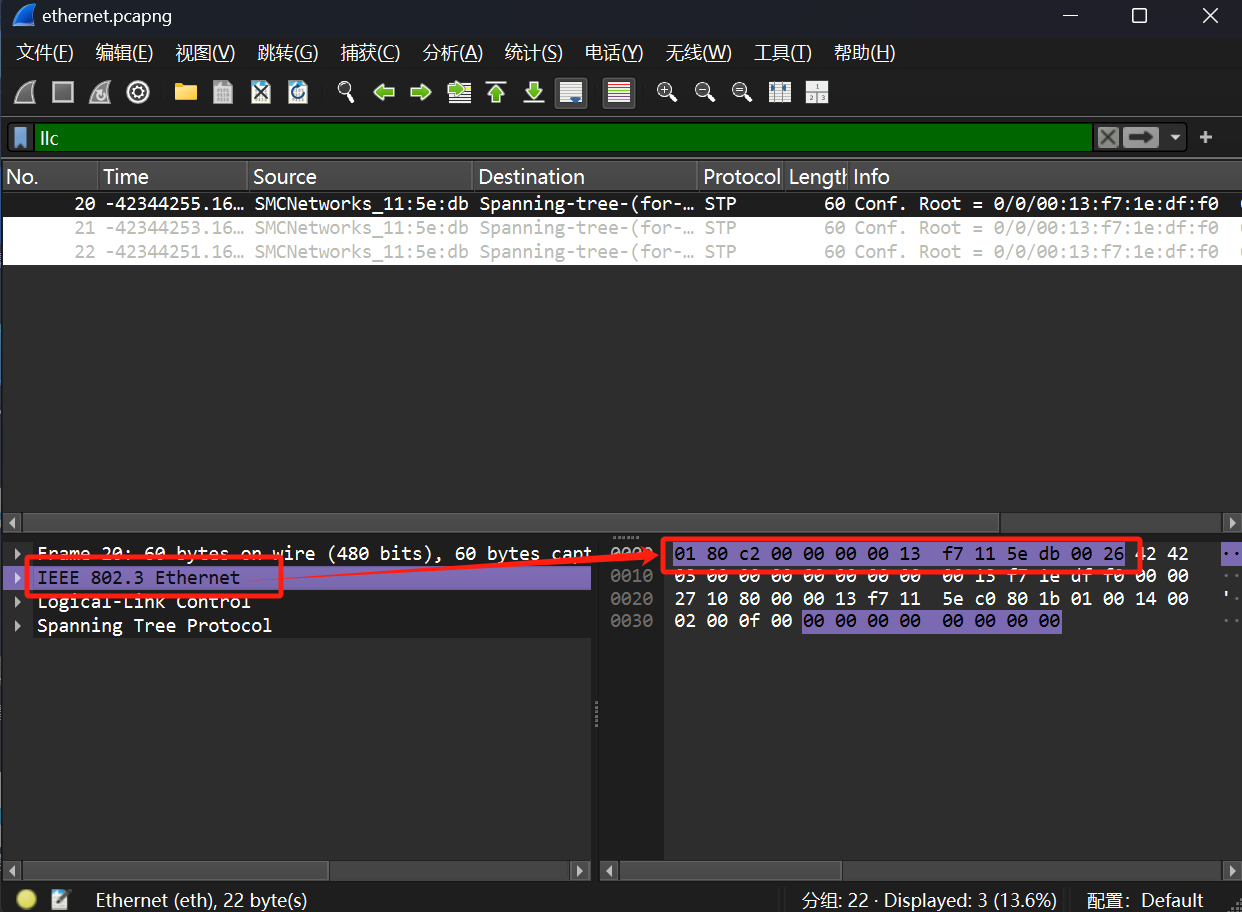
\includegraphics[width=\textwidth]{images/21.IEEE802.3头部.png}
				\caption{IEEE802.3头部}
			\end{minipage}
			\hfill
			\begin{minipage}[b]{0.45\textwidth}
				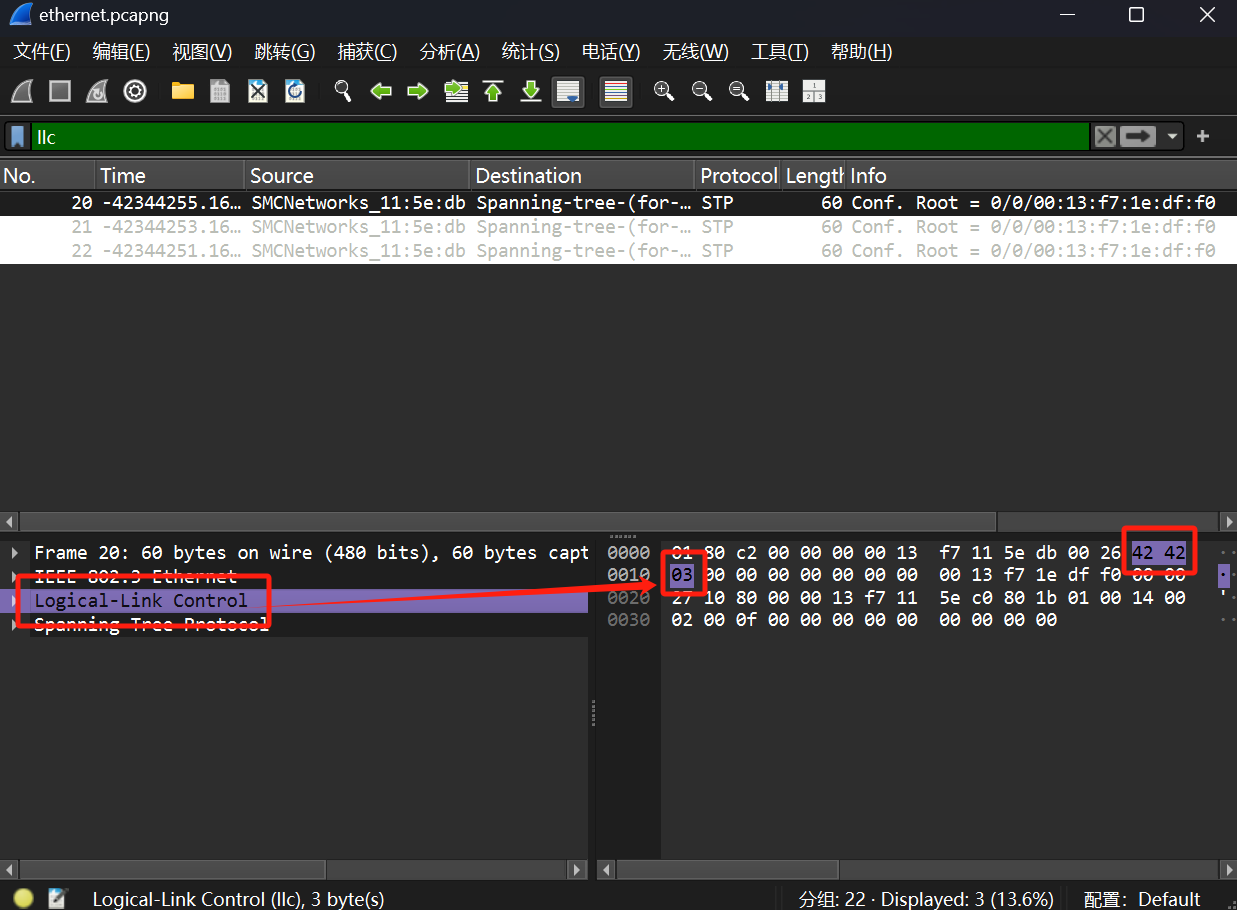
\includegraphics[width=\textwidth]{images/22.LLC头部.png}
				\caption{\texttt{LLC头部}}
			\end{minipage}
		\end{figure}
		
		\item How does the receiving computer know whether the frame is DIX Ethernet or IEEE 802.3? Hint: you may need to both use Wireshark to look at packet examples and read your text near where the Ethernet formats are described.\\
		
		根据\textbf{Type/Length}字段,如果该字段的值小于或等于\texttt{1500},则表示\textbf{Length},为\textbf{IEEE 802.3},否则表示\textbf{Type},为\textbf{DIX}以太网。
		
		\begin{figure}[H]
			\centering
			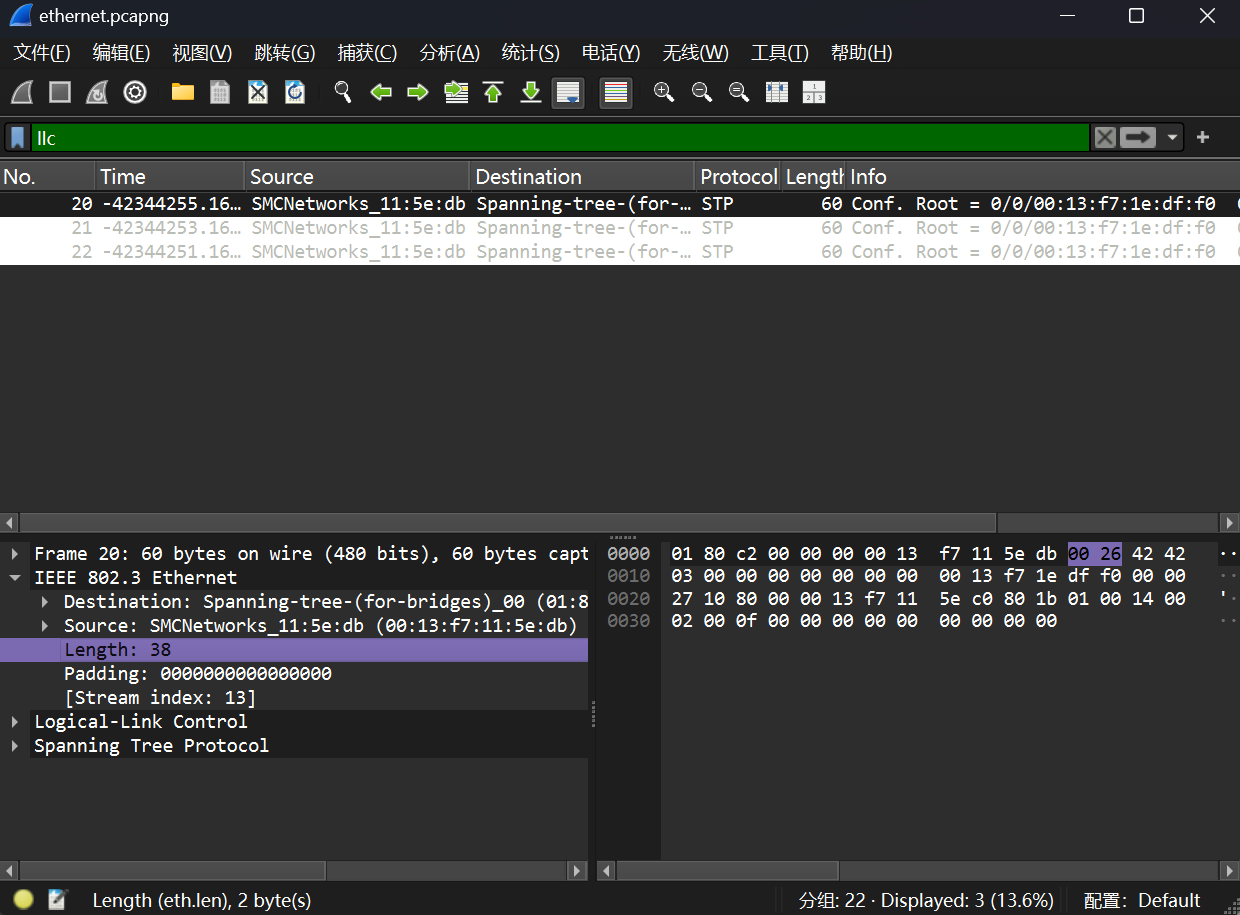
\includegraphics[width=9cm]{images/23.Length字段.png}
			\caption{Length字段}
		\end{figure}
		
		\item If IEEE 802.3 has no Type field, then how is the next higher layer determined? Use Wireshark to look for the demultiplexing key.\\
		
		\textbf{LLC}头中的\textbf{DSAP}字段可以指示上层协议。例如,此处\textbf{DSAP}字段为\textbf{0x42},则表示上层协议为\textbf{STP}。
		
		\begin{figure}[H]
			\centering
			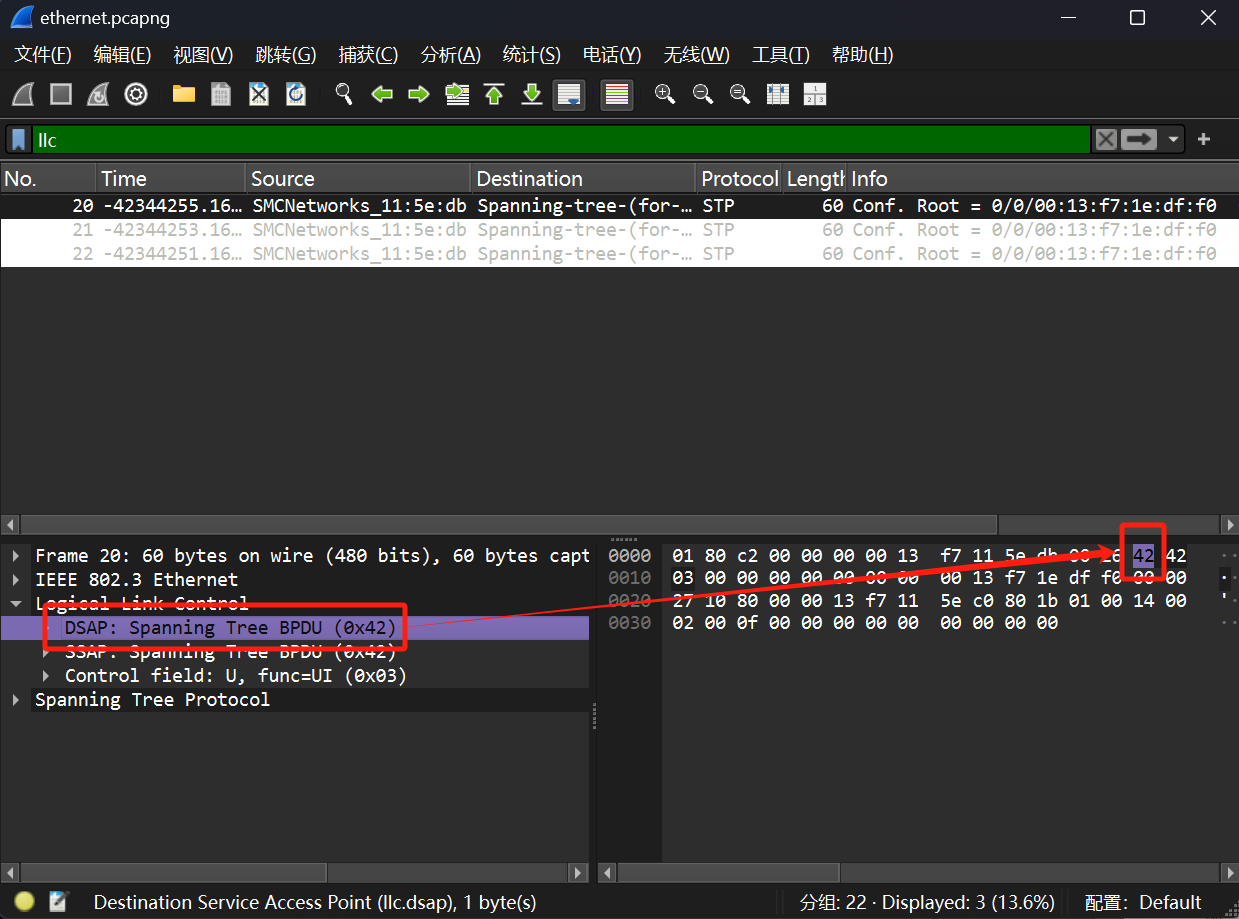
\includegraphics[width=9cm]{images/24.DSAP字段.png}
			\caption{DSAP字段}
		\end{figure}
		
	\end{enumerate}
	
	\section{实验结果总结}
	
	本次实验中,通过使用\textbf{Wireshark}工具,我不仅学会了如何捕获以太网帧,还深入理解了以太网帧的结构。我详细分析了以太网地址的分配范围,并探究了广播帧的工作机制。此外,我对\textbf{DIX}以太网标准和\textbf{IEEE 802.3}标准之间的差异有了更清晰的认识。通过这些学习和探索,我增强了对网络通信协议的理解和应用能力。
	
	\section{附录}
	
	无
	
\end{document}